% Created by tikzDevice version 0.12.4 on 2023-07-12 06:59:59
% !TEX encoding = UTF-8 Unicode
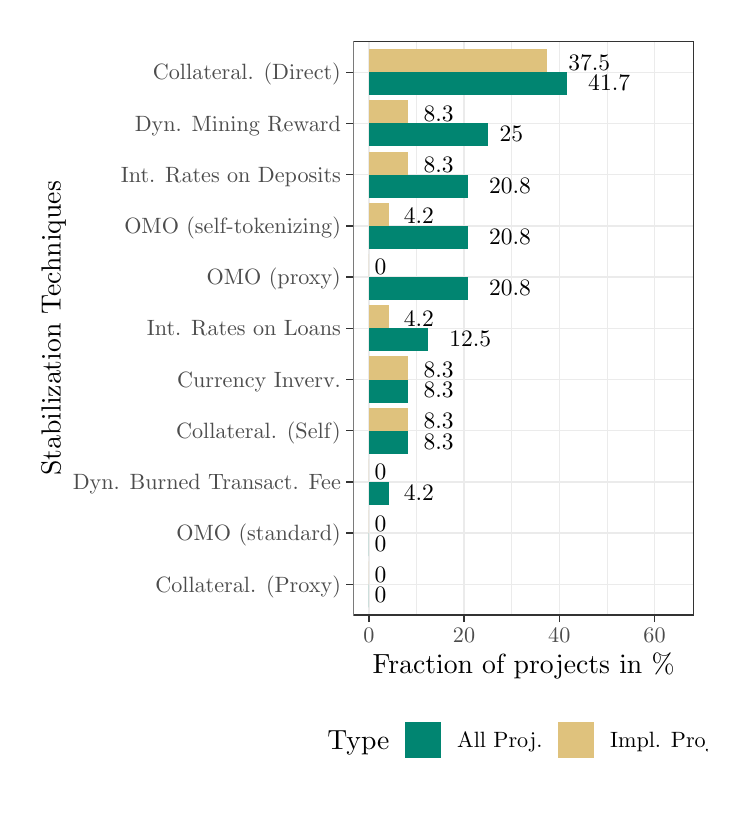
\begin{tikzpicture}[x=1pt,y=1pt]
\definecolor{fillColor}{RGB}{255,255,255}
\path[use as bounding box,fill=fillColor,fill opacity=0.00] (0,0) rectangle (245.72,274.63);
\begin{scope}
\path[clip] (  0.00,  0.00) rectangle (245.72,274.63);
\definecolor{drawColor}{RGB}{255,255,255}
\definecolor{fillColor}{RGB}{255,255,255}

\path[draw=drawColor,line width= 0.5pt,line join=round,line cap=round,fill=fillColor] ( -0.00,  0.00) rectangle (245.72,274.63);
\end{scope}
\begin{scope}
\path[clip] (117.67, 62.35) rectangle (240.72,269.63);
\definecolor{fillColor}{RGB}{255,255,255}

\path[fill=fillColor] (117.67, 62.35) rectangle (240.72,269.63);
\definecolor{drawColor}{gray}{0.92}

\path[draw=drawColor,line width= 0.3pt,line join=round] (140.48, 62.35) --
	(140.48,269.63);

\path[draw=drawColor,line width= 0.3pt,line join=round] (174.89, 62.35) --
	(174.89,269.63);

\path[draw=drawColor,line width= 0.3pt,line join=round] (209.31, 62.35) --
	(209.31,269.63);

\path[draw=drawColor,line width= 0.5pt,line join=round] (117.67, 73.45) --
	(240.72, 73.45);

\path[draw=drawColor,line width= 0.5pt,line join=round] (117.67, 91.96) --
	(240.72, 91.96);

\path[draw=drawColor,line width= 0.5pt,line join=round] (117.67,110.47) --
	(240.72,110.47);

\path[draw=drawColor,line width= 0.5pt,line join=round] (117.67,128.97) --
	(240.72,128.97);

\path[draw=drawColor,line width= 0.5pt,line join=round] (117.67,147.48) --
	(240.72,147.48);

\path[draw=drawColor,line width= 0.5pt,line join=round] (117.67,165.99) --
	(240.72,165.99);

\path[draw=drawColor,line width= 0.5pt,line join=round] (117.67,184.49) --
	(240.72,184.49);

\path[draw=drawColor,line width= 0.5pt,line join=round] (117.67,203.00) --
	(240.72,203.00);

\path[draw=drawColor,line width= 0.5pt,line join=round] (117.67,221.51) --
	(240.72,221.51);

\path[draw=drawColor,line width= 0.5pt,line join=round] (117.67,240.02) --
	(240.72,240.02);

\path[draw=drawColor,line width= 0.5pt,line join=round] (117.67,258.52) --
	(240.72,258.52);

\path[draw=drawColor,line width= 0.5pt,line join=round] (123.27, 62.35) --
	(123.27,269.63);

\path[draw=drawColor,line width= 0.5pt,line join=round] (157.69, 62.35) --
	(157.69,269.63);

\path[draw=drawColor,line width= 0.5pt,line join=round] (192.10, 62.35) --
	(192.10,269.63);

\path[draw=drawColor,line width= 0.5pt,line join=round] (226.52, 62.35) --
	(226.52,269.63);
\definecolor{fillColor}{RGB}{1,133,113}

\path[fill=fillColor] (123.27,250.19) rectangle (194.98,258.52);

\path[fill=fillColor] (123.27, 65.13) rectangle (123.27, 73.45);

\path[fill=fillColor] (123.27,120.65) rectangle (137.60,128.97);

\path[fill=fillColor] (123.27,139.15) rectangle (137.60,147.48);

\path[fill=fillColor] (123.27,157.66) rectangle (144.78,165.99);

\path[fill=fillColor] (123.27,213.18) rectangle (159.11,221.51);

\path[fill=fillColor] (123.27, 83.63) rectangle (123.27, 91.96);

\path[fill=fillColor] (123.27,176.17) rectangle (159.11,184.49);

\path[fill=fillColor] (123.27,194.67) rectangle (159.11,203.00);

\path[fill=fillColor] (123.27,231.69) rectangle (166.29,240.02);

\path[fill=fillColor] (123.27,102.14) rectangle (130.44,110.47);
\definecolor{fillColor}{RGB}{223,194,125}

\path[fill=fillColor] (123.27,258.52) rectangle (187.80,266.85);

\path[fill=fillColor] (123.27, 73.45) rectangle (123.27, 81.78);

\path[fill=fillColor] (123.27,128.97) rectangle (137.60,137.30);

\path[fill=fillColor] (123.27,147.48) rectangle (137.60,155.81);

\path[fill=fillColor] (123.27,165.99) rectangle (130.44,174.32);

\path[fill=fillColor] (123.27,221.51) rectangle (137.60,229.84);

\path[fill=fillColor] (123.27, 91.96) rectangle (123.27,100.29);

\path[fill=fillColor] (123.27,184.49) rectangle (123.27,192.82);

\path[fill=fillColor] (123.27,203.00) rectangle (130.44,211.33);

\path[fill=fillColor] (123.27,240.02) rectangle (137.60,248.34);

\path[fill=fillColor] (123.27,110.47) rectangle (123.27,118.80);
\definecolor{drawColor}{RGB}{0,0,0}

\node[text=drawColor,anchor=base west,inner sep=0pt, outer sep=0pt, scale=  0.85] at (202.56,251.88) {41.7};

\node[text=drawColor,anchor=base west,inner sep=0pt, outer sep=0pt, scale=  0.85] at (125.40, 66.81) {0};

\node[text=drawColor,anchor=base west,inner sep=0pt, outer sep=0pt, scale=  0.85] at (143.05,122.33) {8.3};

\node[text=drawColor,anchor=base west,inner sep=0pt, outer sep=0pt, scale=  0.85] at (143.05,140.84) {8.3};

\node[text=drawColor,anchor=base west,inner sep=0pt, outer sep=0pt, scale=  0.85] at (152.36,159.35) {12.5};

\node[text=drawColor,anchor=base west,inner sep=0pt, outer sep=0pt, scale=  0.85] at (166.70,214.87) {20.8};

\node[text=drawColor,anchor=base west,inner sep=0pt, outer sep=0pt, scale=  0.85] at (125.40, 85.32) {0};

\node[text=drawColor,anchor=base west,inner sep=0pt, outer sep=0pt, scale=  0.85] at (166.70,177.85) {20.8};

\node[text=drawColor,anchor=base west,inner sep=0pt, outer sep=0pt, scale=  0.85] at (166.70,196.36) {20.8};

\node[text=drawColor,anchor=base west,inner sep=0pt, outer sep=0pt, scale=  0.85] at (170.56,233.37) {25};

\node[text=drawColor,anchor=base west,inner sep=0pt, outer sep=0pt, scale=  0.85] at (135.90,103.83) {4.2};

\node[text=drawColor,anchor=base west,inner sep=0pt, outer sep=0pt, scale=  0.85] at (195.39,259.28) {37.5};

\node[text=drawColor,anchor=base west,inner sep=0pt, outer sep=0pt, scale=  0.85] at (125.40, 74.22) {0};

\node[text=drawColor,anchor=base west,inner sep=0pt, outer sep=0pt, scale=  0.85] at (143.05,129.74) {8.3};

\node[text=drawColor,anchor=base west,inner sep=0pt, outer sep=0pt, scale=  0.85] at (143.05,148.24) {8.3};

\node[text=drawColor,anchor=base west,inner sep=0pt, outer sep=0pt, scale=  0.85] at (135.90,166.75) {4.2};

\node[text=drawColor,anchor=base west,inner sep=0pt, outer sep=0pt, scale=  0.85] at (143.05,222.27) {8.3};

\node[text=drawColor,anchor=base west,inner sep=0pt, outer sep=0pt, scale=  0.85] at (125.40, 92.72) {0};

\node[text=drawColor,anchor=base west,inner sep=0pt, outer sep=0pt, scale=  0.85] at (125.40,185.26) {0};

\node[text=drawColor,anchor=base west,inner sep=0pt, outer sep=0pt, scale=  0.85] at (135.90,203.76) {4.2};

\node[text=drawColor,anchor=base west,inner sep=0pt, outer sep=0pt, scale=  0.85] at (143.05,240.78) {8.3};

\node[text=drawColor,anchor=base west,inner sep=0pt, outer sep=0pt, scale=  0.85] at (125.40,111.23) {0};
\definecolor{drawColor}{gray}{0.20}

\path[draw=drawColor,line width= 0.5pt,line join=round,line cap=round] (117.67, 62.35) rectangle (240.72,269.63);
\end{scope}
\begin{scope}
\path[clip] (  0.00,  0.00) rectangle (245.72,274.63);
\definecolor{drawColor}{gray}{0.30}

\node[text=drawColor,anchor=base east,inner sep=0pt, outer sep=0pt, scale=  0.80] at (113.17, 70.70) {Collateral. (Proxy)};

\node[text=drawColor,anchor=base east,inner sep=0pt, outer sep=0pt, scale=  0.80] at (113.17, 89.21) {OMO (standard)};

\node[text=drawColor,anchor=base east,inner sep=0pt, outer sep=0pt, scale=  0.80] at (113.17,107.71) {Dyn. Burned Transact. Fee};

\node[text=drawColor,anchor=base east,inner sep=0pt, outer sep=0pt, scale=  0.80] at (113.17,126.22) {Collateral. (Self)};

\node[text=drawColor,anchor=base east,inner sep=0pt, outer sep=0pt, scale=  0.80] at (113.17,144.73) {Currency Inverv.};

\node[text=drawColor,anchor=base east,inner sep=0pt, outer sep=0pt, scale=  0.80] at (113.17,163.23) {Int. Rates on Loans};

\node[text=drawColor,anchor=base east,inner sep=0pt, outer sep=0pt, scale=  0.80] at (113.17,181.74) {OMO (proxy)};

\node[text=drawColor,anchor=base east,inner sep=0pt, outer sep=0pt, scale=  0.80] at (113.17,200.25) {OMO (self-tokenizing)};

\node[text=drawColor,anchor=base east,inner sep=0pt, outer sep=0pt, scale=  0.80] at (113.17,218.75) {Int. Rates on Deposits};

\node[text=drawColor,anchor=base east,inner sep=0pt, outer sep=0pt, scale=  0.80] at (113.17,237.26) {Dyn. Mining Reward};

\node[text=drawColor,anchor=base east,inner sep=0pt, outer sep=0pt, scale=  0.80] at (113.17,255.77) {Collateral. (Direct)};
\end{scope}
\begin{scope}
\path[clip] (  0.00,  0.00) rectangle (245.72,274.63);
\definecolor{drawColor}{gray}{0.20}

\path[draw=drawColor,line width= 0.5pt,line join=round] (115.17, 73.45) --
	(117.67, 73.45);

\path[draw=drawColor,line width= 0.5pt,line join=round] (115.17, 91.96) --
	(117.67, 91.96);

\path[draw=drawColor,line width= 0.5pt,line join=round] (115.17,110.47) --
	(117.67,110.47);

\path[draw=drawColor,line width= 0.5pt,line join=round] (115.17,128.97) --
	(117.67,128.97);

\path[draw=drawColor,line width= 0.5pt,line join=round] (115.17,147.48) --
	(117.67,147.48);

\path[draw=drawColor,line width= 0.5pt,line join=round] (115.17,165.99) --
	(117.67,165.99);

\path[draw=drawColor,line width= 0.5pt,line join=round] (115.17,184.49) --
	(117.67,184.49);

\path[draw=drawColor,line width= 0.5pt,line join=round] (115.17,203.00) --
	(117.67,203.00);

\path[draw=drawColor,line width= 0.5pt,line join=round] (115.17,221.51) --
	(117.67,221.51);

\path[draw=drawColor,line width= 0.5pt,line join=round] (115.17,240.02) --
	(117.67,240.02);

\path[draw=drawColor,line width= 0.5pt,line join=round] (115.17,258.52) --
	(117.67,258.52);
\end{scope}
\begin{scope}
\path[clip] (  0.00,  0.00) rectangle (245.72,274.63);
\definecolor{drawColor}{gray}{0.20}

\path[draw=drawColor,line width= 0.5pt,line join=round] (123.27, 59.85) --
	(123.27, 62.35);

\path[draw=drawColor,line width= 0.5pt,line join=round] (157.69, 59.85) --
	(157.69, 62.35);

\path[draw=drawColor,line width= 0.5pt,line join=round] (192.10, 59.85) --
	(192.10, 62.35);

\path[draw=drawColor,line width= 0.5pt,line join=round] (226.52, 59.85) --
	(226.52, 62.35);
\end{scope}
\begin{scope}
\path[clip] (  0.00,  0.00) rectangle (245.72,274.63);
\definecolor{drawColor}{gray}{0.30}

\node[text=drawColor,anchor=base,inner sep=0pt, outer sep=0pt, scale=  0.80] at (123.27, 52.34) {0};

\node[text=drawColor,anchor=base,inner sep=0pt, outer sep=0pt, scale=  0.80] at (157.69, 52.34) {20};

\node[text=drawColor,anchor=base,inner sep=0pt, outer sep=0pt, scale=  0.80] at (192.10, 52.34) {40};

\node[text=drawColor,anchor=base,inner sep=0pt, outer sep=0pt, scale=  0.80] at (226.52, 52.34) {60};
\end{scope}
\begin{scope}
\path[clip] (  0.00,  0.00) rectangle (245.72,274.63);
\definecolor{drawColor}{RGB}{0,0,0}

\node[text=drawColor,anchor=base,inner sep=0pt, outer sep=0pt, scale=  1.00] at (179.20, 41.40) {Fraction of projects in \%};
\end{scope}
\begin{scope}
\path[clip] (  0.00,  0.00) rectangle (245.72,274.63);
\definecolor{drawColor}{RGB}{0,0,0}

\node[text=drawColor,rotate= 90.00,anchor=base,inner sep=0pt, outer sep=0pt, scale=  1.00] at ( 11.89,165.99) {Stabilization Techniques};
\end{scope}
\begin{scope}
\path[clip] (  0.00,  0.00) rectangle (245.72,274.63);
\definecolor{fillColor}{RGB}{255,255,255}

\path[fill=fillColor] (103.26,  5.00) rectangle (255.13, 29.45);
\end{scope}
\begin{scope}
\path[clip] (  0.00,  0.00) rectangle (245.72,274.63);
\definecolor{drawColor}{RGB}{0,0,0}

\node[text=drawColor,anchor=base west,inner sep=0pt, outer sep=0pt, scale=  1.00] at (108.26, 13.78) {Type};
\end{scope}
\begin{scope}
\path[clip] (  0.00,  0.00) rectangle (245.72,274.63);
\definecolor{fillColor}{RGB}{255,255,255}

\path[fill=fillColor] (135.75, 10.00) rectangle (150.21, 24.45);
\end{scope}
\begin{scope}
\path[clip] (  0.00,  0.00) rectangle (245.72,274.63);
\definecolor{fillColor}{RGB}{1,133,113}

\path[fill=fillColor] (136.46, 10.71) rectangle (149.50, 23.74);
\end{scope}
\begin{scope}
\path[clip] (  0.00,  0.00) rectangle (245.72,274.63);
\definecolor{fillColor}{RGB}{255,255,255}

\path[fill=fillColor] (191.00, 10.00) rectangle (205.45, 24.45);
\end{scope}
\begin{scope}
\path[clip] (  0.00,  0.00) rectangle (245.72,274.63);
\definecolor{fillColor}{RGB}{223,194,125}

\path[fill=fillColor] (191.71, 10.71) rectangle (204.74, 23.74);
\end{scope}
\begin{scope}
\path[clip] (  0.00,  0.00) rectangle (245.72,274.63);
\definecolor{drawColor}{RGB}{0,0,0}

\node[text=drawColor,anchor=base west,inner sep=0pt, outer sep=0pt, scale=  0.80] at (155.21, 14.47) {All Proj.};
\end{scope}
\begin{scope}
\path[clip] (  0.00,  0.00) rectangle (245.72,274.63);
\definecolor{drawColor}{RGB}{0,0,0}

\node[text=drawColor,anchor=base west,inner sep=0pt, outer sep=0pt, scale=  0.80] at (210.45, 14.47) {Impl. Proj.};
\end{scope}
\end{tikzpicture}
